\documentclass[../masters.tex]{subfiles}

\begin{document}
\graphicspath{{./imgs/}{../imgs/}} %look for images

\section{CSTR Model}
In this section we introduce the model we will use to illustrate the techniques we develop in this dissertation. The model is a simple continuously stirred tank reactor (CSTR) undergoing an exothermic, irreversible first order reaction where $A \rightarrow B$. A schematic diagram of the reactor is shown in Figure \ref{fig_cstr_diagram}. The model is taken from literature \cite{cstrmodel}.
\begin{figure}[H] 
\centering
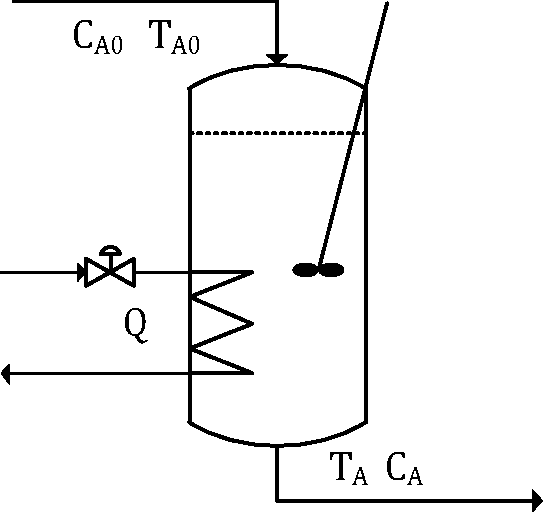
\includegraphics[scale=0.8]{cstr_diagram.pdf}
\caption{Diagram of a simple CSTR where the heat added to system is the only manipulated variable.}
\label{fig_cstr_diagram}
\end{figure}
The state space equations describing the reactor are shown in (\ref{eq_cstrmodel}) with parameters shown in Table \ref{tab_params}. The meaning of the variables is what one would expect from an intuitive understanding: $C_A$ is the concentration of species $A$, $T_R$ is the temperature of the CSTR and $Q$ is the heat added (or removed for negative $Q$) from the CSTR.
\begin{equation}
\begin{aligned}
\dot{C_A} &= \frac{F}{V}\left( C_{A0}-C_A \right) - k_0e^{\frac{-E}{RT_R}}C_A \\
\dot{T_R} &= \frac{F}{V}\left(T_{A0}-T_A\right) + \frac{-\triangle H}{\rho C_p}k_0e^{\frac{-E}{RT_R}}C_A + \frac{Q}{\rho C_p V}
\end{aligned}
\label{eq_cstrmodel}
\end{equation}
\begin{table}[H]
\begin{center}
\begin{tabular}{c c c c}
\hline
$V$ & $~5.0~m^3$ & $R$ & $~8.314~\frac{kJ}{kmol.K}$ \\
$C_{A0}$ & $~1.0~\frac{kmol}{m^3}$ &$T_{A0}$ & $~310~K$ \\
$\triangle H$ & $~-4.78\times 10^{4}~\frac{kJ}{kmol}$ & $k_{0}$ & $~72\times 10^{7}~\frac{1}{min}$ \\
$E$ & $~8.314\times 10^4~\frac{kJ}{kmol}$ & $C_{p}$ & $~0.239~\frac{kJ}{kg.K}$ \\
$\rho$ & $~1000~\frac{kg}{m^3}$ & 
$F$ & $~100\times 10^{-3}~\frac{m^3}{min}$ \\
\hline
\end{tabular}
\caption{CSTR parameters}
\label{tab_params}
\end{center}
\end{table}
The CSTR model is a familiar control example. Similar models may be found in \cite{du}\cite{cervantes}\cite{pan}\cite{yazdi}. We use this model because it is low dimensional yet complex enough to illustrate the principles we investigate. Note that we have increased the volume of the reactor and reduced the rate constant from the reactor we quoted in literature. This is primarily to adjust the time scale of the transient response to be in the order of minutes and not milliseconds.

\subsection{Qualitative Analysis}
In this section we use standard mathematical tools, as found in \cite{edwardsandpenny}, to analyse the qualitative behaviour of the CSTR. By inspecting (\ref{eq_cstrmodel}) we see that the model is coupled and non-linear. By solving (\ref{eq_cstr_statpoints}) we see that for nominal operating conditions ($Q = 0$) there exist 3 operating points (critical points) as shown in Table \ref{tab_nominalstats}.
\begin{equation}
\begin{aligned}
0&= \frac{F}{V}\left( C_{A0}-C_A \right) - k_0e^{\frac{-E}{RT_R}}C_A \\
0 &= \frac{F}{V}\left(T_{A0}-T_A\right) + \frac{-\triangle H}{\rho C_p}k_0e^{\frac{-E}{RT_R}}C_A + \frac{Q}{\rho C_p V}
\end{aligned}
\label{eq_cstr_statpoints}
\end{equation}
\begin{table}[H]
\begin{center}
\begin{tabular}{c c c c}
\hline
Critical Point & $C_A$ & $T_R$ & Stability\\
\hline
$\left(C_A, T_R\right)_0^1$ & 0.0097 & 508.0562 & Stable Improper Node\\
$\left(C_A, T_R\right)_0^2$ & 0.4893 & 412.1302 & Unstable Saddle Point \\
$\left(C_A, T_R \right)_0^3$ & 0.9996 & 310.0709 & Stable Improper Node \\
\hline
\end{tabular}
\caption{Nominal operating points for  the CSTR}
\label{tab_nominalstats}
\end{center}
\end{table}
The stability of the operating points were found by linearising (\ref{eq_cstrmodel}) and computing the eigenvalues of the Jacobian, shown in (\ref{eq_jacobian}), at each critical point.
\begin{equation}
J(C_A, T_R) = \begin{pmatrix}
-\frac{F}{V} - k_0e^{\frac{-E}{RT_R}} & - k_0e^{\frac{-E}{RT_R}}C_A\left(\frac{E}{RT_R^2}\right) \\
\frac{-\triangle H}{\rho C_p}k_0e^{\frac{-E}{RT_R}} & -\frac{F}{V} + \frac{-\triangle H}{\rho C_p}k_0e^{\frac{-E}{RT_R}}C_A\left(\frac{E}{RT_R^2}\right) 
\end{pmatrix}
\label{eq_jacobian}
\end{equation}
In Figure \ref{fig_cstr_op_curve} we see the operating curve for the CSTR. The curve resembles the classical CSTR operating curve with all the associated potential control complexity e.g. input multiplicity etc. \cite{luyben}.
\begin{figure}[H] 
\centering
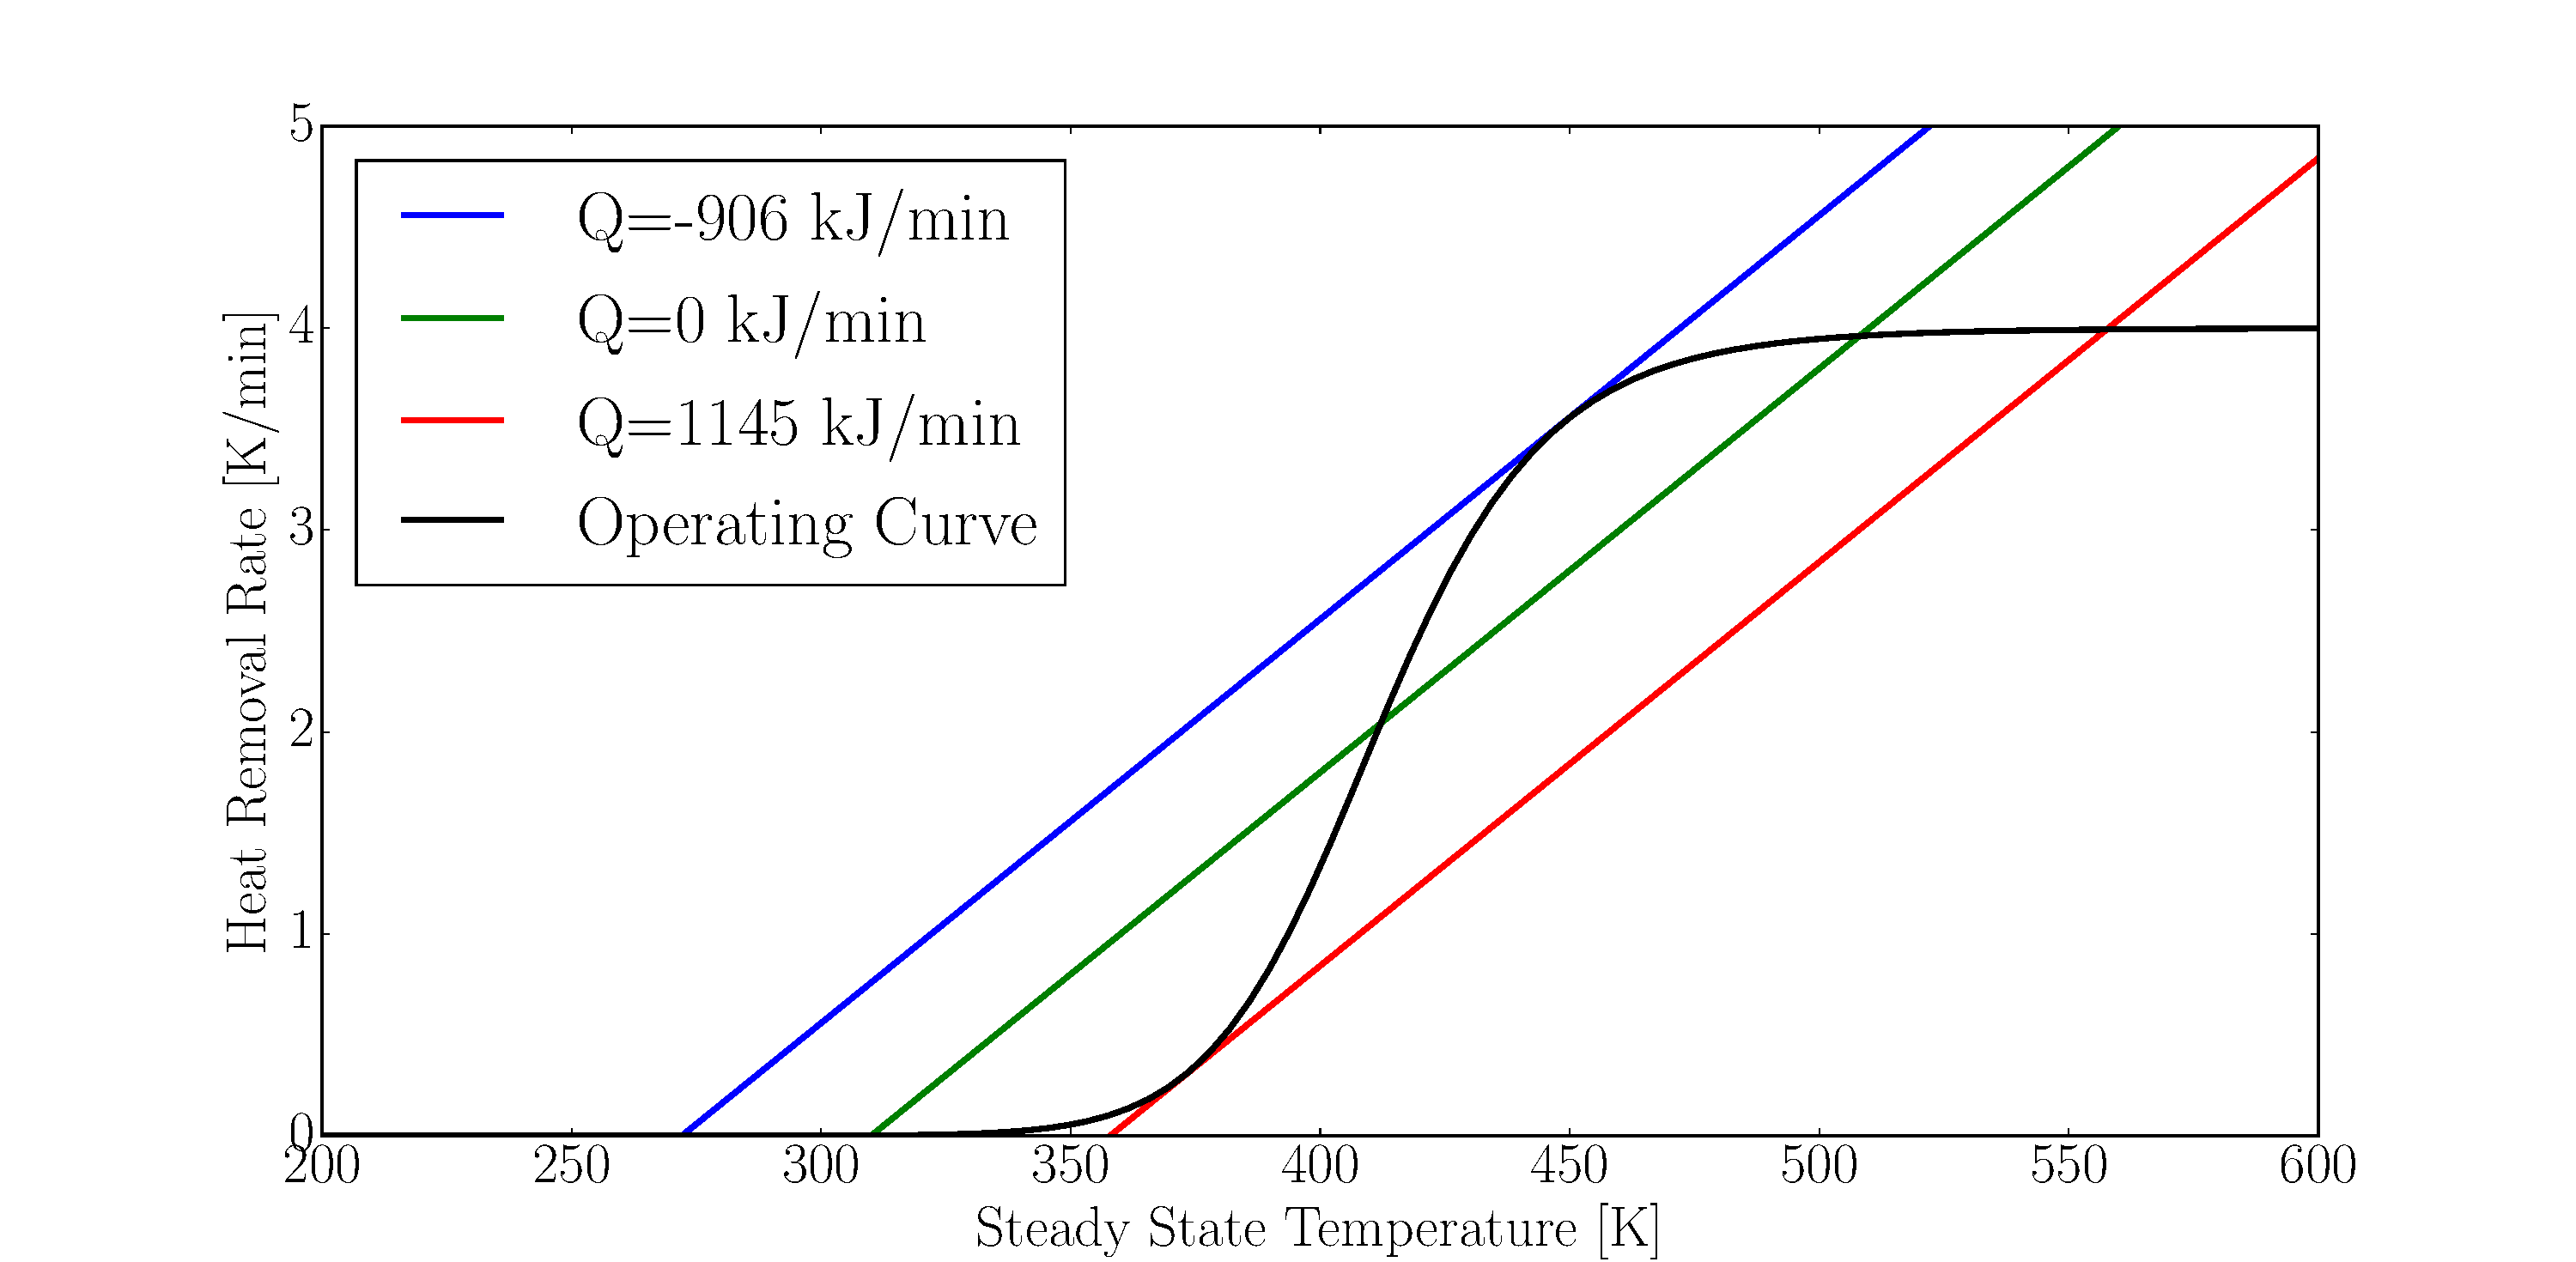
\includegraphics[scale=0.3]{cstr_model_op_curve.pdf}
\caption{CSTR operating curve. Lower heat input to the CSTR drives the system to the low temperature stable operating point and higher heat input drives the CSTR to the higher temperature stable operating point.}
\label{fig_cstr_op_curve}
\end{figure}

\subsection{Nonlinear Model}
In this section we simulate the CSTR

\subsection{Linearised Models}
The approach of using piecewise affine (linear) functions for control, based on linearisation around critical points, has been investigated in literature \cite{du}\cite{kvasnica}. Typically the state domain is discretised into regimes and the linear approximation of the model in each regime is used for control. The benefit of this approach is that the non-linear problem  can then be handled by linear methods for which efficient algorithms exist. A potential drawback of this approach is computational complexity \cite{du}.


\bibliographystyle{plain}
\bibliography{research}

\end{document}